% =================================================================================================
% File:			client_tier.tex
% Description:	Defiinisce la sezione relativa al front-end dell'applicazione
% Created:		2015-03-27
% Author:		Tesser Paolo
% Email:		tesser.paolo@mashup-unipd.it
% =================================================================================================
% Modification History:
% Version		Modifier Date		Change											Author
% 0.0.1 		2015-03-27 			creato scheletro								Tesser Paolo
% =================================================================================================
% 0.0.2			2015-03-28			inserito scheletro del package					Tesser Paolo
% =================================================================================================
% 0.0.3			2015-04-04			inseriti padri dei package e pack contenuti		Tesser Paolo
% =================================================================================================
%

% CONTENUTO DEL CAPITOLO

\subsection{Client (Front-end)} % (fold)
\label{sub:client}
Nel descrivere le componenti si parlerà di classi, che però saranno da intendersi nella loro accezione logica. Il linguaggio di programmazione impiegato infatti non possiede la struttura di classe, ma solo di oggetto, sarà quindi compito del codificatore riportare le classi di seguito identificate nelle strutture fornite dallo specifico linguaggio.

	\subsubsection{bdsm\_app::client} % (fold)
	\label{ssub:bdsm_app_client}
	\begin{figure}[htbp]
		\centering
		\centerline{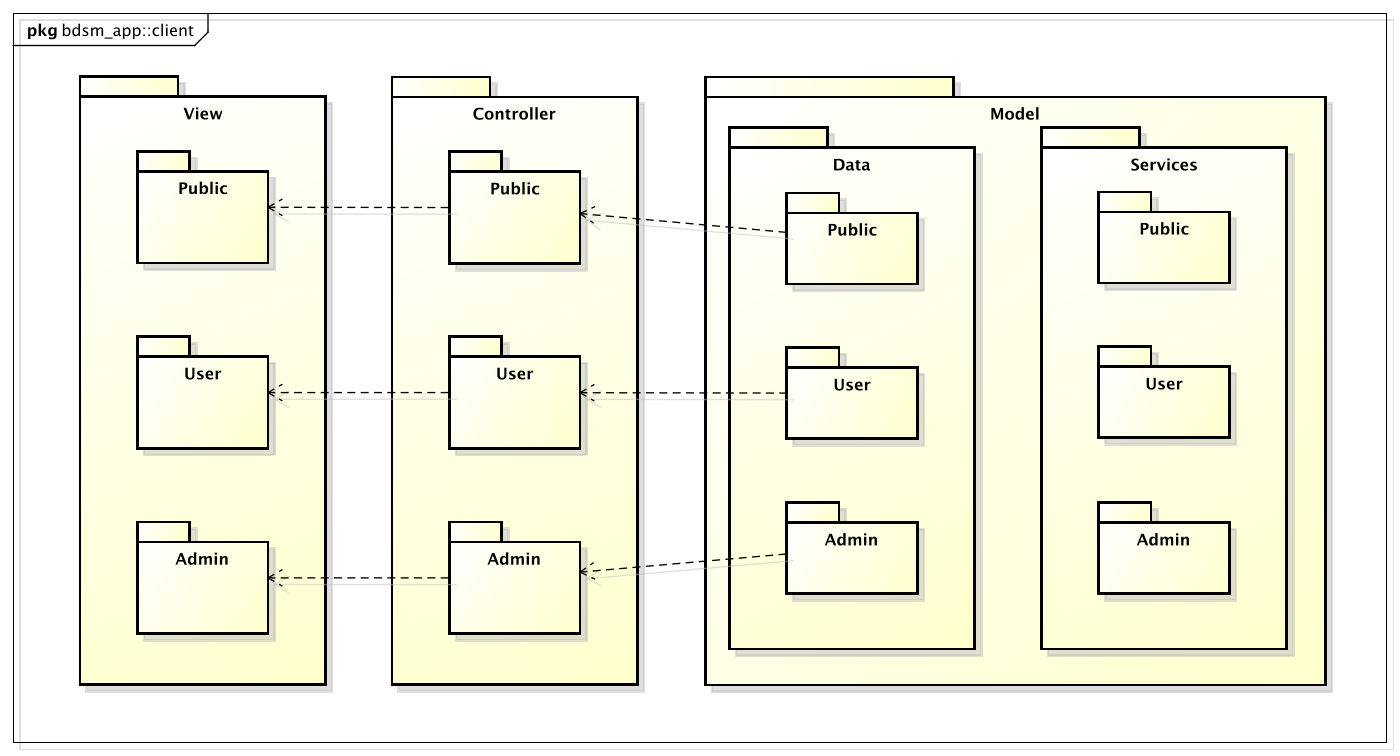
\includegraphics[scale=0.4]{./images/client.pdf}}
		\caption{Package - client}
	\end{figure}
	
	\begin{itemize}
		\item \textbf{Descrizione}: è il package che racchiude tutte le parti del front-end. \'E quindi l'insieme dei componenti che viene eseguito nel browser degli utenti normali e degli amministratori, fornendo loro un'interfaccia grafica per interagire con il sistema;
		\item \textbf{Package contenuti}:
			\begin{itemize}
				\item *::client::model;
				\item *::client::view;
				\item *::client::controller.
			\end{itemize}
		\item \textbf{Interazione con altri componenti}: interagisce con il server definito nella sezione [TO DO] effettuando delle chiamate ai servizi REST offerti;
	\end{itemize}
	% subsubsection bdsm_app_client (end)

	\pagebreak
	% PACKAGE MODEL

	\subsubsection{bdsm\_app::client::model} % (fold)
	\label{ssub:bdsm_app_client_model}
	[TO DO] (diagramma) \newline \newline

	\begin{itemize}
		\item \textbf{Descrizione}: [TO DO];
		\item \textbf{Padre}: client;
		\item \textbf{Package contenuti}:
			\begin{itemize}
				\item client::model::data;
				\item client::model::services.
			\end{itemize}
		\item \textbf{Interazione con altri componenti}: [TO DO];
	\end{itemize}
	% subsubsection bdsm_app_client_model (end)


	\subsubsection{bdsm\_app::client::model::data} % (fold)
	\label{ssub:bdsm_app_client_model_data}
	[TO DO] (diagramma) \newline \newline

	\begin{itemize}
		\item \textbf{Descrizione}: [TO DO];
		\item \textbf{Padre}: client::model;
		\item \textbf{Package contenuti}:
			\begin{itemize}
				\item client::model::data::public;
				\item client::model::data::user;
				\item client::model::data::admin.
			\end{itemize}
		\item \textbf{Interazione con altri componenti}: [TO DO];
	\end{itemize}
	% subsubsection bdsm_app_client_model_data (end)

	\subsubsection{bdsm\_app::client::model::data::public} % (fold)
	\label{ssub:bdsm_app_client_model_data_public}
	[TO DO] (diagramma) \newline \newline

	\begin{itemize}
		\item \textbf{Descrizione}: [TO DO];
		\item \textbf{Padre}: client::model::data;
		\item \textbf{Interazione con altri componenti}: [TO DO];
	\end{itemize}

		\paragraph{Classi} % (fold)
			\subparagraph{Nome package::Nome classe} % (fold)
			\label{subp:subparagraph_name}
				\begin{itemize}
					\item \textbf{Descrizione}: [TO DO];
					\item \textbf{Utilizzo}: [TO DO];
					\item \textbf{Classi ereditate}: [TO DO];
					\item \textbf{Relazioni con altre classi}: [TO DO].
				\end{itemize}	
	% subsubsection bdsm_app_client_model_data_public (end)

	\subsubsection{bdsm\_app::client::model::data::user} % (fold)
	\label{ssub:bdsm_app_client_model_data_user}
	[TO DO] (diagramma) \newline \newline

	\begin{itemize}
		\item \textbf{Descrizione}: [TO DO];
		\item \textbf{Padre}: client::model::data;
		\item \textbf{Interazione con altri componenti}: [TO DO];
	\end{itemize}

		\paragraph{Classi} % (fold)
			\subparagraph{Nome package::Nome classe} % (fold)
			\label{subp:subparagraph_name}
				\begin{itemize}
					\item \textbf{Descrizione}: [TO DO];
					\item \textbf{Utilizzo}: [TO DO];
					\item \textbf{Classi ereditate}: [TO DO];
					\item \textbf{Relazioni con altre classi}: [TO DO].
				\end{itemize}	
	% subsubsection bdsm_app_client_model_data_user (end)

	\subsubsection{bdsm\_app::client::model::data::admin} % (fold)
	\label{ssub:bdsm_app_client_model_data_admin}
	[TO DO] (diagramma) \newline \newline

	\begin{itemize}
		\item \textbf{Descrizione}: [TO DO];
		\item \textbf{Padre}: client::model::data;
		\item \textbf{Interazione con altri componenti}: [TO DO];
	\end{itemize}

		\paragraph{Classi} % (fold)
			\subparagraph{Nome package::Nome classe} % (fold)
			\label{subp:subparagraph_name}
				\begin{itemize}
					\item \textbf{Descrizione}: [TO DO];
					\item \textbf{Utilizzo}: [TO DO];
					\item \textbf{Classi ereditate}: [TO DO];
					\item \textbf{Relazioni con altre classi}: [TO DO].
				\end{itemize}	
	% subsubsection bdsm_app_client_model_data_admin (end)


	\subsubsection{bdsm\_app::client::model::services} % (fold)
	\label{ssub:bdsm_app_client_model_services}
	[TO DO] (diagramma) \newline \newline

	\begin{itemize}
		\item \textbf{Descrizione}: [TO DO];
		\item \textbf{Padre}: client::model;
		\item \textbf{Package contenuti}:
			\begin{itemize}
				\item client::model::services::public;
				\item client::model::services::user;
				\item client::model::services::admin.
			\end{itemize}
		\item \textbf{Interazione con altri componenti}: [TO DO];
	\end{itemize}
	% subsubsection bdsm_app_client_model_services (end)

	\subsubsection{bdsm\_app::client::model::services::public} % (fold)
	\label{ssub:bdsm_app_client_model_services_public}
	[TO DO] (diagramma) \newline \newline

	\begin{itemize}
		\item \textbf{Descrizione}: [TO DO];
		\item \textbf{Padre}: client::model::services;
		\item \textbf{Interazione con altri componenti}: [TO DO];
	\end{itemize}

		\paragraph{Classi} % (fold)
			\subparagraph{Nome package::Nome classe} % (fold)
			\label{subp:subparagraph_name}
				\begin{itemize}
					\item \textbf{Descrizione}: [TO DO];
					\item \textbf{Utilizzo}: [TO DO];
					\item \textbf{Classi ereditate}: [TO DO];
					\item \textbf{Relazioni con altre classi}: [TO DO].
				\end{itemize}	
	% subsubsection bdsm_app_client_model_services_public (end)

	\subsubsection{bdsm\_app::client::model::user} % (fold)
	\label{ssub:bdsm_app_client_model_user}
	[TO DO] (diagramma) \newline \newline

	\begin{itemize}
		\item \textbf{Descrizione}: [TO DO];
		\item \textbf{Padre}: client::model::services;
		\item \textbf{Interazione con altri componenti}: [TO DO];
	\end{itemize}

		\paragraph{Classi} % (fold)
			\subparagraph{Nome package::Nome classe} % (fold)
			\label{subp:subparagraph_name}
				\begin{itemize}
					\item \textbf{Descrizione}: [TO DO];
					\item \textbf{Utilizzo}: [TO DO];
					\item \textbf{Classi ereditate}: [TO DO];
					\item \textbf{Relazioni con altre classi}: [TO DO].
				\end{itemize}	
	% subsubsection bdsm_app_client_model_user (end)

	\subsubsection{bdsm\_app::client::model::services::admin} % (fold)
	\label{ssub:bdsm_app_client_model_services_admin}
	[TO DO] (diagramma) \newline \newline

	\begin{itemize}
		\item \textbf{Descrizione}: [TO DO];
		\item \textbf{Padre}: client::model::services;
		\item \textbf{Interazione con altri componenti}: [TO DO];
	\end{itemize}

		\paragraph{Classi} % (fold)
			\subparagraph{Nome package::Nome classe} % (fold)
			\label{subp:subparagraph_name}
				\begin{itemize}
					\item \textbf{Descrizione}: [TO DO];
					\item \textbf{Utilizzo}: [TO DO];
					\item \textbf{Classi ereditate}: [TO DO];
					\item \textbf{Relazioni con altre classi}: [TO DO].
				\end{itemize}	
	% subsubsection bdsm_app_client_model_services_admin (end)






	% END PACKAGE MODEL
	\pagebreak
	% PACKAGE DELLA VIEW

	\subsubsection{bdsm\_app::client::view} % (fold)
	\label{ssub:bdsm_app_client_view}
	\begin{figure}[htbp]
		\centering
		\centerline{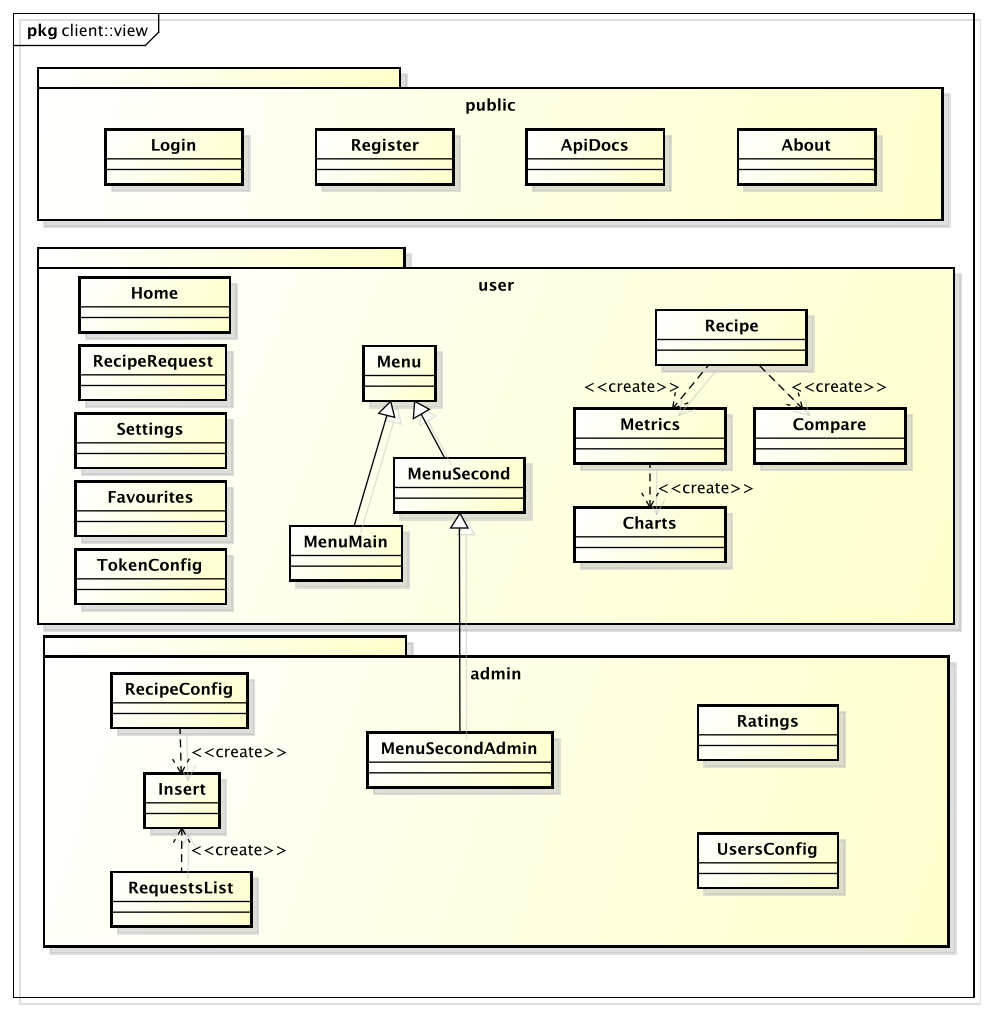
\includegraphics[scale=0.45]{./images/client_view.pdf}}
		\caption{Package - client::view}
	\end{figure}

	\begin{itemize}
		\item \textbf{Descrizione}: [TO DO];
		\item \textbf{Padre}: client;
		\item \textbf{Package contenuti}:
			\begin{itemize}
				\item client::view::public;
				\item client::view::user;
				\item client::view::admin.
			\end{itemize}
		\item \textbf{Interazione con altri componenti}: [TO DO];
	\end{itemize}
	% subsubsection bdsm_app_client_view (end)

	\subsubsection{bdsm\_app::client::view::public} % (fold)
	\label{ssub:bdsm_app_client_view_public}
	\begin{figure}[htbp]
		\centering
		\centerline{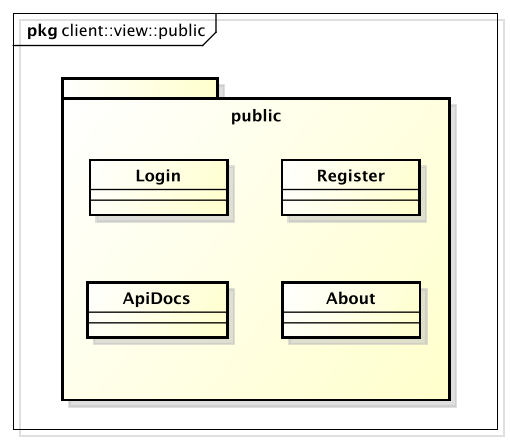
\includegraphics[scale=0.6]{./images/client_view_public.pdf}}
		\caption{Package - client::view::public}
	\end{figure}

	\begin{itemize}
		\item \textbf{Descrizione}: [TO DO];
		\item \textbf{Padre}: client::view;
		\item \textbf{Interazione con altri componenti}: [TO DO];
	\end{itemize}

		\paragraph{Classi} % (fold)
			\subparagraph{Nome package::Nome classe} % (fold)
			\label{subp:subparagraph_name}
				\begin{itemize}
					\item \textbf{Descrizione}: [TO DO];
					\item \textbf{Utilizzo}: [TO DO];
					\item \textbf{Classi ereditate}: [TO DO];
					\item \textbf{Relazioni con altre classi}: [TO DO].
				\end{itemize}
	% subsubsection bdsm_app_client_view_public (end)


	\subsubsection{bdsm\_app::client::view::user} % (fold)
	\label{ssub:bdsm_app_client_view_user}
	\begin{figure}[htbp]
		\centering
		\centerline{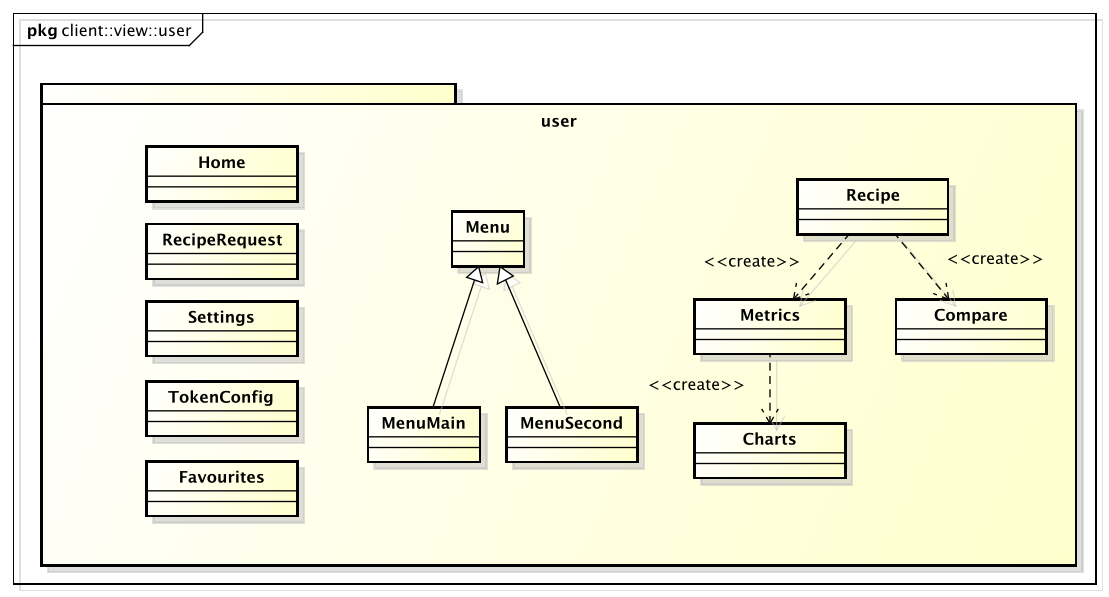
\includegraphics[scale=0.45]{./images/client_view_user.pdf}}
		\caption{Package - client::view::user}
	\end{figure}

	\begin{itemize}
		\item \textbf{Descrizione}: [TO DO];
		\item \textbf{Padre}: client::view;
		\item \textbf{Interazione con altri componenti}: [TO DO];
	\end{itemize}

		\paragraph{Classi} % (fold)
			\subparagraph{Nome package::Nome classe} % (fold)
			\label{subp:subparagraph_name}
				\begin{itemize}
					\item \textbf{Descrizione}: [TO DO];
					\item \textbf{Utilizzo}: [TO DO];
					\item \textbf{Classi ereditate}: [TO DO];
					\item \textbf{Relazioni con altre classi}: [TO DO].
				\end{itemize}
	% subsubsection bdsm_appclient__view_user (end)

	\subsubsection{bdsm\_app::client::view::admin} % (fold)
	\label{ssub:bdsm_app_client_view_admin}
	\begin{figure}[htbp]
		\centering
		\centerline{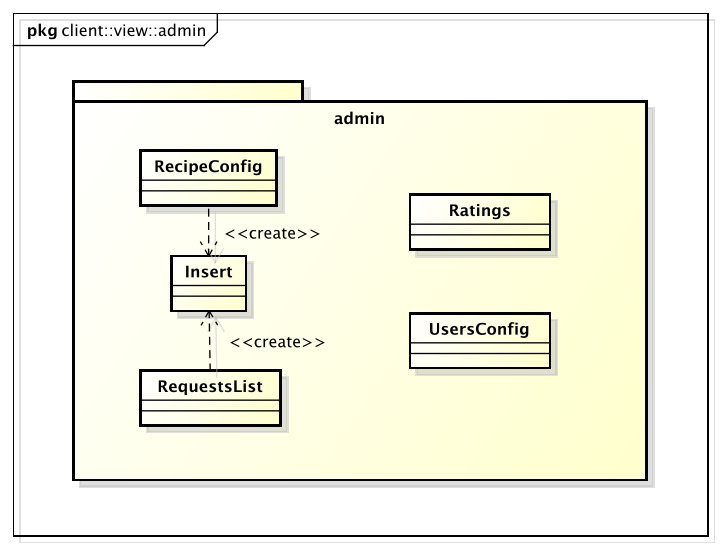
\includegraphics[scale=0.5]{./images/client_view_admin.pdf}}
		\caption{Package - client::view::admin}
	\end{figure}

	\begin{itemize}
		\item \textbf{Descrizione}: [TO DO];
		\item \textbf{Padre}: client::view;
		\item \textbf{Interazione con altri componenti}: [TO DO];
	\end{itemize}

		\paragraph{Classi} % (fold)
			\subparagraph{Nome package::Nome classe} % (fold)
			\label{subp:subparagraph_name}
				\begin{itemize}
					\item \textbf{Descrizione}: [TO DO];
					\item \textbf{Utilizzo}: [TO DO];
					\item \textbf{Classi ereditate}: [TO DO];
					\item \textbf{Relazioni con altre classi}: [TO DO].
				\end{itemize}
	% subsubsection bdsm_app_client_view_admin (end)

	% END PACKAGE VIEW
	\pagebreak
	% PACKAGE CONTROLLER

	\subsubsection{bdsm\_app::client::controller} % (fold)
	\label{ssub:bdsm_app_client_controller}
	[TO DO] (diagramma) \newline \newline

	\begin{itemize}
		\item \textbf{Descrizione}: [TO DO];
		\item \textbf{Padre}: client;
		\item \textbf{Package contenuti}:
			\begin{itemize}
				\item client::controller::public;
				\item client::controller::user;
				\item client::controller::admin.
			\end{itemize}
		\item \textbf{Interazione con altri componenti}: [TO DO];
	\end{itemize}
	% subsubsection bdsm_app_client_controller (end)


	\subsubsection{bdsm\_app::client::controller::public} % (fold)
	\label{ssub:bdsm_app_client_controller_public}
	[TO DO] (diagramma) \newline \newline

	\begin{itemize}
		\item \textbf{Descrizione}: [TO DO];
		\item \textbf{Padre}: client::controller;
		\item \textbf{Interazione con altri componenti}: [TO DO];
	\end{itemize}

		\paragraph{Classi} % (fold)
			\subparagraph{Nome package::Nome classe} % (fold)
			\label{subp:subparagraph_name}
				\begin{itemize}
					\item \textbf{Descrizione}: [TO DO];
					\item \textbf{Utilizzo}: [TO DO];
					\item \textbf{Classi ereditate}: [TO DO];
					\item \textbf{Relazioni con altre classi}: [TO DO].
				\end{itemize}
	% subsubsection bdsm_app_client_controller_public (end)



	\subsubsection{bdsm\_app::client::controller::user} % (fold)
	\label{ssub:bdsm_app_client_controller_user}
	[TO DO] (diagramma) \newline \newline

	\begin{itemize}
		\item \textbf{Descrizione}: [TO DO];
		\item \textbf{Padre}: client::controller;
		\item \textbf{Interazione con altri componenti}: [TO DO];
	\end{itemize}

		\paragraph{Classi} % (fold)
			\subparagraph{Nome package::Nome classe} % (fold)
			\label{subp:subparagraph_name}
				\begin{itemize}
					\item \textbf{Descrizione}: [TO DO];
					\item \textbf{Utilizzo}: [TO DO];
					\item \textbf{Classi ereditate}: [TO DO];
					\item \textbf{Relazioni con altre classi}: [TO DO].
				\end{itemize}
	% subsubsection bdsm_app_client_controller_user (end)

	\subsubsection{bdsm\_app::client::controller::admin} % (fold)
	\label{ssub:bdsm_app_client_controller_admin}
	[TO DO] (diagramma) \newline \newline

	\begin{itemize}
		\item \textbf{Descrizione}: [TO DO];
		\item \textbf{Padre}: client::controller;
		\item \textbf{Interazione con altri componenti}: [TO DO];
	\end{itemize}

		\paragraph{Classi} % (fold)
			\subparagraph{Nome package::Nome classe} % (fold)
			\label{subp:subparagraph_name}
				\begin{itemize}
					\item \textbf{Descrizione}: [TO DO];
					\item \textbf{Utilizzo}: [TO DO];
					\item \textbf{Classi ereditate}: [TO DO];
					\item \textbf{Relazioni con altre classi}: [TO DO].
				\end{itemize}
	% subsubsection bdsm_app_client_controller_admin (end)

	% END PACKAGE CONTROLLER



	% TEMPLATE PER IL PACKAGE
	\subsubsection{Nome package} % (fold)
	\label{ssub:nome_del_package}
	[TO DO] (diagramma) \newline \newline

	\begin{itemize}
		\item \textbf{Descrizione}: [TO DO];
		\item \textbf{Padre}: [TO DO] (qualora presente);
		\item \textbf{Package contenuti}: [TO DO] (qualora presente);
		\item \textbf{Interazione con altri componenti}: [TO DO];
	\end{itemize}

		\paragraph{Classi} % (fold)
			\subparagraph{Nome package::Nome classe} % (fold)
			\label{subp:subparagraph_name}
				\begin{itemize}
					\item \textbf{Descrizione}: [TO DO];
					\item \textbf{Utilizzo}: [TO DO];
					\item \textbf{Classi ereditate}: [TO DO];
					\item \textbf{Relazioni con altre classi}: [TO DO].
				\end{itemize}
			% subparagraph subparagraph_name (end)

			% subsection nome_classe (end)

		% paragraph classi (end)
	% subsubsection nome_del_package (end)

% subsection client (end)